\documentclass[10pt,twocolumn]{article}

\usepackage{times}
\usepackage{fullpage}
\usepackage{listings}
\usepackage{graphicx}
\usepackage{multirow}
\usepackage{clrscode3e}
\usepackage{epsfig,subfigure,framed}
\usepackage{refstyle,amsmath,chngcntr}


\begin{document}

\title{\bf Detecting RCU bugs using Software Watchpoint}
\author{Akshay Kumar and Dhaval Giani }
\date{}
\maketitle
\thispagestyle{empty}

\lstset{language=C,basicstyle=\ttfamily,tabsize=4, columns=fullflexible}
\begin{abstract}
Application debugging is a tedious chore in software development cycle. The need of an efficient debugger increases with the complexity of software involving parallel system. Read Copy Update (RCU) is a wait-free synchronization mechanism which gets heavily used in the parallel system to reduce overheads and avoid deadlocks. Being complex in its design, one needs to take a lot of care while using RCU. The incorrect usage of RCU often leads to programming error or bugs. The existing solution for analysing such bugs are imprecise and generate false positive. 

In this project we introduces a new approach for analysing such bugs using \emph{Software Watchpoint}. Our \emph{Watchpoint} mechanism is implemented using Dynamic Binary Instrumentation (DBI) technique and provides efficient infrastructure to enforce memory access policy. We used \emph{Watchpoint} to track and verify the references of RCU protected data. Our system is precise and imposes moderate overhead for reader and low overhead for writer thread. Our system is limited in its approach and identify bugs related to pointer leak in classical RCU. 

\end{abstract}

\section{Introduction}\label{sec:intro}
Parallel programming is already mainstream these days. There are a wide variety
of mechanisms being used to provide synchronization and serialization.
Operating systems are a popular example for utilizing various synchronization
mechanims%Add citations here for spinlocks, mutexes and for RCU, with possibly links to the sourcse as opposed to publications for Linux/BSD/Solaris
With scalability being extremely important for the Operating Systems,
techniques have been proposed to reduce the overheads by utilizing lock-free
techniques. Read Copy Update~\cite{paulmck:TechReport} is one such technique which is
heavily used in the Linux Kernel. RCU has been described as a publish-subscribe
technique.

In its simplest form, readers disable preemption when they enter the RCU read critical
section and reenable premption while exiting the
critical section. A sample implementation can be seen in Figure ~\ref{fig:rcusimpleread}.
On the other hand updaters synchronize with the use
of one of the traditional mechanisms such as spin locks or mutexes while updating.
Following an update, any new readers gets to access the updated version. However
readers who came in before the update was `published` would still be guaranteed
to the see the older version which is reclaimed only after all the pre-existing
readers have gone away.

\begin{figure}[h]
\centering
\begin{lstlisting}
#define rcu_read_lock	preempt_disable
#define rcu_read_unlock	preempt_enable
\end{lstlisting}
\caption{A simple implementation of RCU read side primitives}\label{fig:rcusimpleread}
\end{figure}

RCU is becoming increasingly relevant today with a userspace implementation also
being released and used~\cite{urcu}.%cite urcu paper and the flocking using RCU paper
~\cite{goulet:thesis},~\cite{urcu-crowd}




\section{Background}\label{sec:back}
Programming with RCU is a completely different paradigm as compared to traditional synchronization techniques. It provides a well defined primitive which can be used for defining critical section, updating or accessing rcu protected data. Due to its complex design, care must be taken while using these rcu synchronization primitive.


Figure~\ref{fig:rwuse} shows an example of typical Reader-Writer lock and how it works. In this example, \emph{q} is shared data which can be accessed by various reader and writer threads. \emph{q\_lock} is a \emph{rwlock\_t} which is used to synchronize the access \emph{q} between different readers and writers. To read \emph{q}, first reader acquires the \emph{rwlock\_t}, \emph{q\_lock}, in read mode. The reader then goes ahead and reads shared data \emph{q}. Once it is done with reading, it unlocks \emph{q\_lock}.

In contrast Figure~\ref{fig:RCUuse} gives an example of RCU synchronization primitive and how it can be used. Here, \emph{q} is a global data shared between various readers \& writers and is protected using RCU. When a reader wishes to dereference that data, it first announces the beginning of an RCU critical section using \emph{rcu\_read\_lock()}. Then in order to dereference \emph{q}, it uses \emph{rcu\_dereference()}. At this point it holds a legal reference and RCU guarantees that structure will not be reclaimed at least until this reader announces the end of the critical section. The reader now go ahead and use the reference it has. Finally once it is done, it announces the end of a critical section with the use of \emph{rcu\_read\_unlock()}.

In the two examples we can see that, as opposed to locking on a rwlock, RCU readers just announce they have entered a critical section. In order to ensure that access is not
interrupted, they use \emph{rcu\_dereference()} to get a reference. Access could be interrupted due to the compiler re-ordering some accesses while optimizing, which might lead
to wrong results. It is also possible for some architectures (notably DEC Alpha) to reorder loads and stores which is also going to lead to an undesirable result. Finally all accesses to the shared data is through the use of \emph{p}. RCU guarantees that the data structure
will not be reclaimed till the reader announces the end of its critical section.

In order to take the discussion further, it is important to introduce two terms that need to be defined in the context of RCU.
\begin{itemize}
\item{\bf Quiescent State}: This is the state when a reader is not in an RCU read critical state.
\item{\bf Grace Period}: Any time period during which each thread has been observed in at least one quiescent state.
\end{itemize}


\begin{figure}[t]
\centering
\begin{lstlisting}
rwlock_t q_lock;
global datatype *q;

f() {
	...
	rwlock_read_lock(&q_lock);
	do_something(q);
	rwlock_read_unlock(&q_lock);
	...
}
\end{lstlisting}
\caption{Using Reader Writer locks}\label{fig:rwuse}
\end{figure}

\begin{figure}[b]
\centering
\begin{lstlisting}
global datatype *q;

f() {
	dataype *p;
	...
	rcu_read_lock();
	p = rcu_dereference(q);
	do_something(p);
	rcu_read_unlock();
	...
}
\end{lstlisting}
\caption{Using RCU}\label{fig:RCUuse}
\end{figure}


RCU also has a list of well defined primitive. The most commonly used are
\begin{itemize}
\item\emph{rcu\_read\_lock}: Used to announce the beginning of a critical section.
\item\emph{rcu\_read\_unlock}: Used to announce the end of a critical section.
\item\emph{rcu\_dereference}: Used to obtain a reference to shared data
\item\emph{rcu\_assign\_pointer}: Used to announce an update.
\item\emph{synchronize\_rcu}: Used to wait till a grace period has passed.
\item\emph{call\_rcu}: Used to queue up a callback that takes place after the end of some grace period that starts in the future.
\end{itemize}


Using RCU requires careful attention from the programmer. There are some rules
and inherent assumptions while using RCU. For example, access to shared data
should only happen with a reference which has been obtained with the use of
\emph{rcu\_dereference()}. This call should also happen only after an RCU read critical
section has announced. Any use of this reference obtained must be made before
this critical section ends. If a new critical section has been announced a
fresh reference must be obtained with the use of \emph{rcu\_dereference()}. A quiescent
state (in some flavours of RCU) must only be announced once it has actually
taken place.~\footnote{It is also important to note that while care must be taken to announce a
quiescent state only when it has actually occured, one must not delay the announcement
of the quiescent state. Since RCU maintains multiple copies which are only reclaimed
after a grace period has occured, it serves only to increase the memory pressure on
the system.} On the update side, an update should only take place with use
of \emph{rcu\_assign\_pointer()}. There are many other similar rules that must be
followed.


\section{Proposal}\label{sec:proposal}
As mentioned in Section~\ref{sec:back} usage of RCU requires a lot of care. One needs to follow many rules while writing code which uses RCU. Figures~\ref{fig:rcuderefbug} and~\ref{fig:rcuusebug} show some examples.

\begin{figure}[h]
\centering
\begin{lstlisting}
f() {
	...
	rcu_read_lock();
	p = q;
	do_something(p);
	rcu_read_unlock();
	...
}
\end{lstlisting}
\caption{RCU bugs: Not using rcu\_derefence}\label{fig:rcuderefbug}
\end{figure}

\begin{figure}[h]
\centering
\begin{lstlisting}
f() {
	...
	rcu_read_lock();
	p = rcu_dereference(q);
	x = p;
	rcu_read_unlock();
	...
	rcu_read_lock();
	do_something(x);
	rcu_read_unlock();
	...
}
\end{lstlisting}
\caption{RCU bugs: Not using in the correct critical section}\label{fig:rcuusebug}
\end{figure}

In figure~\ref{fig:rcuderefbug} a reference to q takes place directly without the use
of \emph{rcu\_dereference()}. Since \emph{rcu\_dereference()} has not been used to
dereference q, the compiler barriers are not in place and therefore the compiler
is free to aggresively speculate pointer values. This may lead to an undesirable
result.

In figure~\ref{fig:rcuusebug}, while p has been obtained with the
use of \emph{rcu\_dereference()}, it is used (in the form of x) after the critical section
has been announced. As the end of a read critical section has been announced,
RCU is now free to reclaim the reference that p may be pointing to. As a result
when p is dereference in the next critical section, that can be a pointer to
garbage which is very undesirable.  A similar bug would be if the reference
obtained was outside the critical section.

Both these examples be broadly class as RCU pointer leaks.

As mentioned in section~\ref{sec:back}, there are many rules that must be followed
while using RCU. For the purposes of this report, we shall name two rules.
\begin{itemize}
\item{\bf Rule 0}: Any access to RCU protected data must happen in an RCU read critical section.
\item{\bf Rule 1}: Any reference to RCU protected data in a read critical section must obtained with the use \emph{rcu\_dereference}
\item{\bf Rule 2}: Any reference obtained \emph{using rcu\_dereference} must be used within the critical section it was obtained in.
\end{itemize}

We shall call the bugs of the type represented in figure~\ref{fig:rcuderefbug} as \emph{Rule 1 violations}
and those in figure~\ref{fig:rcuusebug} as \emph{Rule 2 violations}.
This project aims to detect and report bugs of these two types. Detecting these bugs is extremely challenging. Due to the nature of RCU implementation,
bugs are subtle and at times hard to reproduce. Even though the references have been illegaly obtained, they might still be valid.

In order to detect \emph{Rule 1 violations}, we must first identify data
that has been protected by RCU. We must then be able to track every
dereference to it. We must also be in a position to instrument
every \emph{rcu\_dereference()} call.

For \emph{Rule 2 violations}, we must know when a dereference takes place.
At that point in time, we need to be able to check if the reference has
been obtained legally. If so, we must know if it has been obtained in
the current critical section.





%
%In order to detect these issues, we use \emph{generations}. A \emph{Generation}
%can be defined as an RCU read critical section. A generation has the following
%properties

%\begin{itemize}

%\item \emph{Generations} are per-thread
%\item A new \emph{generation} starts when \emph{rcu\_read\_lock} is called
%\item A \emph{generation} ends when \emph{rcu\_read\_unlock} is called

%\end{itemize}

%To detect these violations, we use \emph{granary} which is described in
%further detail in section~\ref{sec:impl}. Granary provides us the ability
%to add unlimited watchpoints.

%We first identify RCU protected data.
%This can be acheived in a number of ways. The easiest way is to intercept calls
%to \emph{rcu\_assign\_pointer}. A watchpoint is added at that point. The watchpoint
%is \emph{per-pointer}. The watchpoint is erased only when a reclaim takes place.

%Whenever an \emph{rcu\_dereference} takes place, a check is made to confirm that
%a \emph{generation} has started. If not, this detects that an \emph{rcu\_dereference}
%has taken place outside a critical section and is a \emph{rule 2 violation} If a
%generation has started, we then tag the associated RCU pointer with the current
%generation.

%When a dereference of RCU protected data takes place, the very first check is made
%to see if a \emph{generation} has started. The absence of a generation detects
%a \emph{rule 2 violation}.

%Next the RCU pointer must be checked to see if it was legally obtained. This is checked by checking the
%\emph{generation} information of the pointer. Since \emph{generation} information
%is setup only at the point when an \emph{rcu\_dereference} takes place, absence
%of this information indicates a \emph{rule 1 violations}.

%However the presence of the \emph{generation} information does not imply that the RCU
%pointer is legal. In order to confirm that, the \emph{generation} in the RCU pointer is
%compared with current thread's \emph{generation}. If the two generations are the same,
%then the RCU pointer is legal. Any other case denotes a \emph{rule 2 violation}


\section{Approach}\label{sec:appr}
The previous sections describe about the importance of Read Copy Update (RCU) in parallel programming paradigm and rules one should follow to correctly use the RCU primitives. It also describes about the violation of RCU rules, which can be a potential bug in program, and challenges involved in identifying such bugs. There are existing solution like static analysis~\cite{sparse}, lockdep-RCU~\cite{PaulEMcKenney2010LockdepRCU} etc which is used to identify such bugs but they are imprecise and generate false positive.

Our approach to identify the such RCU bugs involves the technique of Dynamic Binary Instrumentation (DBI). Dynamic Binary Instrumentation (DBI) is an execution control and analysis technique that involves injecting binary code into a running program. The injected code is term “Instrumentation”. There are many DBI infrastructure exist like DynamoRIO~\cite{Bruening04efficient}, DynamoRIO Kernel (DRK)~\cite{Feiner:2012:CKI:2150976.2150992},  Pin~\cite{Bungale:2007:PPF:1254810.1254830}, JIFL~\cite{Olszewski:2007:JIN:1272996.1273000}, KernInst~\cite{Tamches:1999:UDK:1080598.1080605} etc which provides support for fine-grained monitoring and program execution. Our system uses Granary~\cite{GranaryAtOSDI}, a comprehensive kernel module instrumentation framework. The choice of Granary as DBI framework is based on the fact that it provides the support for instrumenting only kernel modules and thus incur no overhead when non-module code executes. Granary allows the interaction between the kernel and module through wrappers having rich information about kernel and its types, thus giving us the complete control on all the data passed over it. It also provide the infrastructure for adding watchpoint for all the memory addresses passed over the wrapper. Our decision to use Granary as the DBI framework is also based on the fact that we used rcu torture test module to evaluate our system which needs the instrumentation of only module code. 


\subsection{Granary}
Granary~\cite{GranaryAtOSDI} is a Dynamic Binary Instrumentation (DBI) framework, developed over DynamoRIO Kernel (DRK) and provides support for fine-grained instrumentation of only kernel modules. Granary gets loaded as the kernel module and interposes during module loading mechanism to generate the module wrapper. It also use the rich kernel type informations to generate a static kernel wrapper. Once the module gets loaded, it runs under the control of Granary and all interactions between the kernel and module happens through one of these wrappers. The presence of these wrappers provides an efficient infrastructure to monitor all the pointers passed from the kernel to the module and add watchpoint on them. The rich kernel type information at the wrapper layer provides support for adding type-based watchpoint on the pointers. However for this project we are using simple watchpoint implementation for tracking the use of RCU primitive and access of RCU protected data. The detail of watchpoint implementation and its usage is provided in next section. 


\subsection{Behavioural Watchpoint}
Watchpoints are an integral feature of program analysis and debugging tools because they correlate watched memory locations with the program points accessing those memory locations. There are two categories of watchpoints: hardware-based and software-based. Hardware-based watchpoints are fast but scarce, which limits their usefulness as a means of perfoming large-scale program analyses \cite{UnlimitedWatchpoints}. Software-based implementations can scale to support millions of watchpoints \cite{Zhao:2008}, but are limited by their view of memory as an opaque sequence of bytes. This view is at odds with program analysis tools, which require contextual information about a program's memory. The watchpoint-based analysis tools are harder to design and implement because they must maintain separate bookkeeping mechanisms to recover contextual information about watched memory. These contextual informations are important when used for analysing the access of RCU protected memory. To achieve our goal, we introduce \emph{behavioural watchpoints}: a new form of software-based watchpoints that simplify the context based program analysis and debugging.  Behavioural watchpoints address the usability concerns of hardware-based watchpoints and overcome the incongruency between how software implements watchpoints and how program analysis tools use watchpoints.

Two characteristics define our behavioural watchpoints:
\begin{enumerate}
	\item[i)] Context-specific information is embedded in each watchpoint. This information is directly available and can be updated when watched address is accessed.
	\item[ii)] The action taken when a watched address is accessed is a component of the context-specific information. This implies that different watchpoints can \emph{behave} differently.
\end{enumerate} 

Implementing software based behavioural watchpoint, without any architectural support, is expensive since it requires to inspect all memory operations and trigger a callback based on the context. A naive approach of implementing watchpoints using dynamic binary instrumentation adds new instructions across every memory references to performs the following task: 
\begin{enumerate}
	\item[i)] Determine the list of addresses which needs to be watched and check if the program is referring to one of the watched addresses.  
	\item[ii)] Check the contextual information and raise a callback when memory operation happens at one of the watched addresses.
	\item[iii)] Incase the address is not one of the watched addresses, continue the normal execution.
\end{enumerate} 
 
The naive system maintains a watchlist lookup table to maintain the list of addresses to be watched and uses an efficient algorithm to look for the addresses.% in the list. One of the drawback of this approach is the runtime overhead, which incurs due to address lookup for every memory addresses.  
To achieve our design goal, we implemented watchpoints by adding an extra level of indirection to memory addresses. An unwatched address is converted into a watched address by changing its high-order bits. These high-order bits indirectly identify context-specific information about the range of memory being watched. This information, called the watchpoint's \emph{descriptor}, contains the originating watched address and a set of functions to invoke when watched memory is dereferenced. Since watchpoint information is embedded in only the high-order bits, a typical offset of a watched address is another watched address that shares the same watchpoint-specific high-order bits. A watchpoint's descriptor is indirectly located by interpreting these high-order bits as an index into a global \emph{watchpoint descriptor table} (\Figref{watchpoint_descriptor_table})

Our approach has the following design implications which is useful for debugging the RCU based applications.

%Any unwatched address can be converted into an watched address. The extra level of indirection added by watching an address allows us to efficiently locate context-specific information about the memory being watched.

%A watchpoint is added to a program by changing the high-order order bits of an address used by the program. 
%Watchpoints work on ranges instead of individual units of memory because a watchpoint is added to a program by changing 

\paragraph{A watched address must be distinguishable from an unwatched address.}All watched addresses are non-canonical addresses that trigger a hardware exception when dereferenced. We take advantage of the x86-64 architecture for implementing watched addresses. In kernel space on x86-64, canonical addresses have their 16 high-order bits set to 1. Watched addresses do not take this form. To prevent hardware exceptions, instrumentation is dynamically added to memory loads and stores. Watched addresses are detected before they are dereferenced and resolved to their unwatched counterparts (by masking the 16 high-order bits to 1). An alternative approach is to dereference a watched address and implement behavioural watchpoints in the trap handler.
	
\paragraph{Multiple watchpoints can watch the same range of memory.}Two copies of an address (e.g.,two pointers to the same object) can be separately watched, so long as the pattern of their high-order bits is different. This is useful for distinguishing between logically different objects that occupy the same memory. This features enables the detection of RCU usage bugs involving violation of Rule 1. %For example, this feature enables efficient detection of use-after-free bugs without preventing deallocated memory from being immediately reallocated for another use. This efficiency comes from our ability to have one watchpoint for the freed memory, and another watchpoint for newly allocated memory occupying the same space.
	
\paragraph{Watchpoints are viral.}If an address $A$ is watched, then every address derived from $A$ (e.g. through copying or offsetting) is also watched. This is useful for memory and taint analysis tools: a watchpoint that is added early on in the lifetime of an address (e.g., immediately before the address of some newly allocated memory is returned from an allocator) can persist and propagate until no more derived addresses exist.

\begin{figure}[t]
\begin{center}
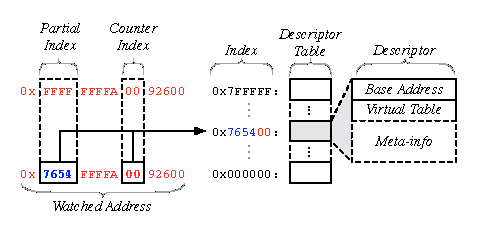
\epsfig{file=watchpoints.eps}
\end{center}
\caption{\label{fig:watchpoint_descriptor_table}A watched address (bottom left) and its corresponding unwatched address (top left) are compared. The process of resolving the watchpoint descriptor for the watched address is shown.}
\end{figure}

\paragraph{Millions of watchpoints are supported.}Our design as described uses 15 of the 16 high-order bits (called the \emph{partial index}) of a watched address for identifying a watchpoint's descriptor. 15 bits only allows 32K watchpoints. To increase the number of watchpoints, we use an additional 8 bits (bits 20-27, called the \emph{counter index}) in the address to index into the watchpoint descriptor table (\Figref{watchpoint_descriptor_table}). This counter index extends the number of possible watchpoints to 8M and is left unchanged when converting an unwatched address into a watched address. The key advantage of our watchpoint scheme is the ability to directly map watched addresses to unwatched addresses using a simple bitmask. The main drawback of the scheme is that an offset of a watched address can cause the low-order bits to overflow into the counter index. We are exploring several solutions to this problem.

%This approach has some drawbacks when an offset of a watched address causes the low-order bits to overflow into the counter index; however, we have several solutions to this problem. 

\paragraph{Watchpoint descriptors can be arbitrarily customized.}This aspect of watchpoints is possible because our design separates the allocation/management of descriptors and the addresses that they watch. Arbitrary extension of descriptors supports our goal of overcoming the incongruency between the needs of debugging an analysis tools (contextual information about watched memory), and how existing software implements watchpoints (watched memory is opaque).

%\subsection{Extensions}
%Our design includes the following extensions to watchpoints, which expand on the behavioural aspect of our watchpoint implementation.
%principally enable the \emph{behavioural} aspect of our software-based watchpoint .
%Our goal of using watchpoints to watch the memory of objects required the following 

%\paragraph{Watchpoints are type-specific.} When a watchpoint is added to an address, the \emph{type} of the address determines what meta-information is included in the descriptor, as well as what functions to invoke when memory watched by the watchpoint is accessed. Two powerful applications of this extension are discussed in \Secref{type_overflow} and \Secref{access_policies}.

%\paragraph{Triggered watchpoint functions are polymorphic.} The function invoked when watched memory is accessed is decided using a descriptor-specific virtual table (vtable). Each vtable provides eight functions: four read and four write functions. Each function is specific to a memory operand size (1, 2, 4, or 8 bytes). A watchpoint descriptor is initialised with either a generic or a type-specific vtable. Type-specific vtables are specific to the \emph{type} of the watched address. Vtables earn behavioural watchpoints their name because they allow watchpoints to behave differently when watched memory is accessed.

%When invoked, a vtable function operates on the watched address and its descriptor. Behavioural watchpoints earn their name from their ability to behave differently based on the meta-information stored in the descriptor and the (type-specific) vtable function invoked.

%\paragraph{Watchpoints remember their originating address.} The address to which a watchpoint is first added is called its \emph{base address}, and is stored in the watchpoint descriptor. We designed watchpoints to remember their base address because it helps to ``anchor" contextual information. When a watchpoint is added, \emph{something} is known about the watched address. Later in a program's execution, an offset of the watched address might be dereferenced. Little can be said about the dereferenced address in relation to the watchpoint's originating address without knowing the originating address.

%Program debugging is a inevitable task in software development process. An efficient debugger can make programmers more productive by allowing them to monitor the execution, inspect the state of the process and monitor memory read and write to inspect the data flow and corruption~\cite{Zhao:2008}. This increases the requirement of an efficient debugging tool supporting an useful feature called \emph{Watchpoints}. The need of such debugging tool increases, as the complexity of the program grows such as parallel system. \emph{Watchpoint} allow a developer to demarcate a memory region and take control whenever that gets accessed. It then ensures the safe access of the memory addresses by checking certain policy. It is similar to the instruction breakpoints which allows the developer to pause execution at specific instructions.

%Implementing software watchpoint, without any architectural support, is expensive since it requires to inspect all memory operations and trigger a callback on the watched addresses. Our system leverages the advances in binary instrumentation and code manipulation technique to provide the efficient feature to add watchpoint at memory addresses. Our system uses this feature to check the correct usage of RCU synchronization primitive and access of RCU protected data, thus identifying the violation of rules and possible buggy usage of RCU.

%The naive approach of implementing watchpoint using dynamic binary instrumentation adds new instructions across every memory references to performs the following task: 
%\begin{itemize}
%	\item Determine the list of addresses which needs to be watched and check if the program is referring to one of the watched addresses.  
%	\item Raise a callback when memory operation happens at one of the watched addresses.
%	\item Incase the address is not one of the watched addresses, continue the normal execution.
%\end{itemize}  
%The naive system also maintains a watchlist lookup table to maintain the list of addresses to be watched. It uses an efficient algorithm to look for the addresses in the list before making a callback on watched addresses. One of the drawback of this approach is the runtime overhead, which incurs due to address lookup for every memory addresses. This makes the implementation of watchpoint costly. 
%\begin{figure}
%\centering
% 	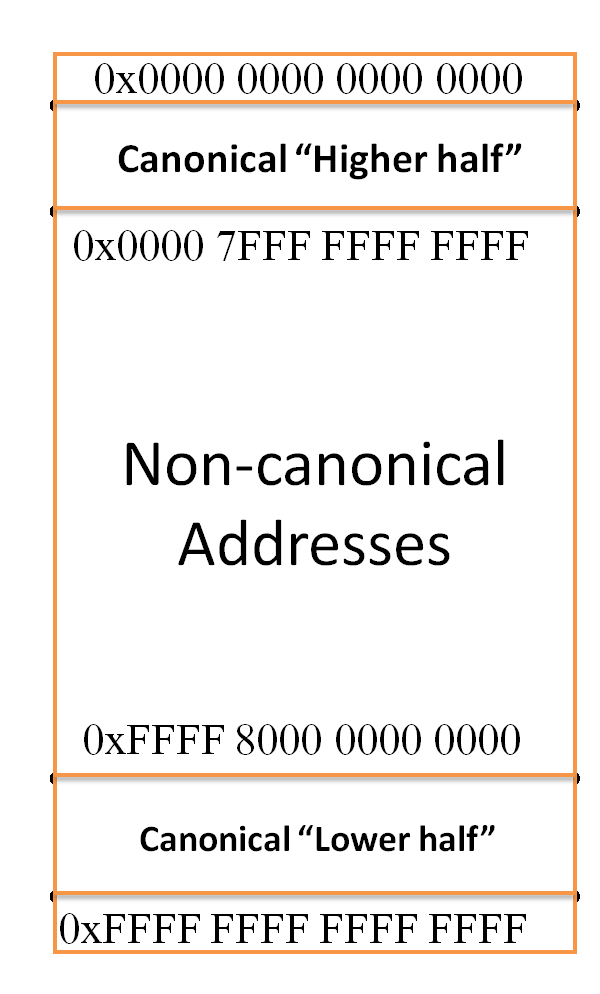
\includegraphics[width=0.2\textwidth]{Picture3-png}
%\caption{64-bit address-space layout (48bit implementation)}\label{fig:addrspace}
%\end{figure}

%Our system refines the cost of adding watchpoint by substantially reducing the cost of lookup and providing options for faster lookup of meta information in shadow memory. The detail about shadow memory and meta information is provided in next section. We took the advantage of 48 bit implementation in 64-bit architecture and used non-canonical addresses to implement our watchpoint mechanism. The use of non-canonical address provides us the following advantages :
%\begin{itemize}
%	\item It decreases the cost of lookup as the non-canonical addresses can be easily recognised by masking lower 48 bits of the addresses.
%	\item It also provides one to one mapping between the actual address and watched address thus proving virtually no cost for fixing the address.
%	\item The unused 15 bits in non-canonical address is used to encode information about the shadow memory storing meta-informations.
%	\item The pointer aliasing the watched address also gets watched, thus there is no need to implement a pointer tracking mechanism.
%\end{itemize}   

%Figure~\ref{fig:addrspace} shows the address-space layout in 64 bit architecture with 48 bit implementations. 
%The highest 1 bit (sign bit) is used for adding watchpoint and differentiate between original and watched addresses. The next 15 bit of address is used to for storing shadow memory index storing meta-information. Our method of storing shadow memory index puts a limit on our system in terms of number of active watchpoint we can add at a time, but we consider this is enough for our project to track the rcu protected data. Figure~\ref{fig:watchpoint} shows the detail, how the watched address gets created.

%\begin{figure}[h]
%\centering
% 	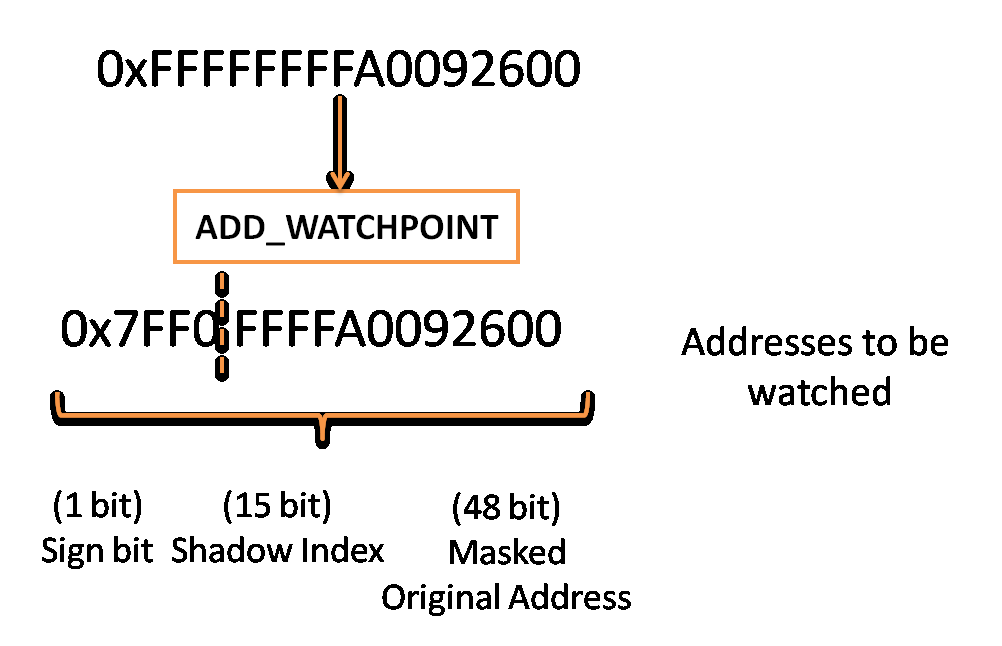
\includegraphics[width=0.4\textwidth]{Picture6-png}
%\caption{Generated Watchpoint Address}\label{fig:watchpoint}
%\end{figure} 

\subsection {Instrumentation and Optimizations}
Watchpoints essentially requires monitoring of every memory read (load) and write (store) operations. A basic monitoring approach using dynamic binary instrumentation adds new instructions before every memory references looking for one of the watched address. %In our system these watched addresses includes non-canonical addresses generated out of original address and the index of shadow memory storing required meta-information. The detail of watchpoint implementation is provided in previous subsection. 
The instrumentation required for implementing watchpoint perform the following operation before every memory references: 

\begin{enumerate}
	\item[i)] Save and restore the registers that are used or side-effected during watchpoint lookup( stack is used to spill these registers ).
	\item[ii)] Calculate the reference address and check if this is one of the non-canonical addresses. Inject a callback function, if the address is one of the non-canonical one. 
	\item[iii)] Emulate the actual instruction with corrected address and continue the execution after restoring registers.
	\item[iv)] Follow the normal course of execution if the address is not one of the watched addresses.
\end{enumerate}

Figure~\ref{fig:mem-write} shows the example of basic instrumentation required for every memory operations. The naive instrumentation suffers from a significant runtime overhead. We implemented and applied some of the optimization to systematically improve the runtime performance. %We used the following optimizations: 
\begin{itemize}
	\item \emph{Dead Registers Analysis:} Every instrumentation system needs scratch registers for creating and injecting new instructions. These registers can be obtained by spilling them to stack or memory locations. %Our naive instrumentation uses stack to spill these registers. 
The frequent spilling of these registers on stack or memory location increases the cost of instrumentation significantly~\cite{Probst02registerliveness, Muth98registerliveness}. Our system performs the register liveness analysis on each basic block to identify registers that can be safely used without requiring it to spill on the stack. For register liveness analysis, our system starts instrumenting from the end of the basicblock moving upward and collecting all the source and destination registers making all the non source and non base-displacement registers (whole destination registers) as dead.  
	\item \emph{Flag Liveness Analysis:} %Instrumentation can change  , we also need to save and restore the flags as the instrumented code modifies the flag. 
One important optimization in instrumentation is Flag Liveness analysis. We save and restore the flag only when it is alive. To identify the dead flag as we move upward instrumenting basic block, we find if any of the instruction modify the flags we consider the instruction previous to that as having dead flag. 
	\item \emph{Merge Checks:} We also exploited the locality of memory references and two instructions in the same basic block accessing the same object or different member of same object (like \emph{0x0(\%rax) and 0x8(\%rax)}) doesn’t require the instrumentation of all references and thus the checks for all of them is merged together.
    \item \emph{Eliminate Stack Operations:} For x86 architecture, any operation on the stack or involving stack pointer is also considered as memory operation. Our system identify all these instructions involving operations on the stack and they are not required to be instrumented since we are not tracking or adding watchpoint on them.
\end{itemize}

\begin{figure}[ht!]
%
\framebox{\begin{minipage}[t]{1.02\columnwidth}%
\vspace{-1em}
\begin{codebox}
\Procname{$\proc{Native-Memory-Operation}$}
\li  mov $\id{\%rsi   -> [\%rax, \%rbx]}$ 
\end{codebox}%

\begin{codebox}
\Procname{$\proc{Instrumented-Memory-Operation}$}
\li  	push 	$\id{\%rcx}$
\li  	push 	$\id{\%rdi}$
\li 	lea 	$\id{[\%rax, \%rbx] 	-> 	\%rdi}$
\li 	pushf
\li 	movabs 	$\id{0xffff000000000000		->	\%rcx}$
\li	or 	$\id{\%rcx 	->	\%rdi}$
\li	cmp 	$\id{\%rdi 	->	\%rdi}$
\li	je     	$\id{addr\_not\_watchpoint}$
\li	popf
\li 	$\proc{insert\_clean\_call}(\id{watch\_write}, \id{\%rdi}, \id{1})$
\li	mov    	$\id{\%rsi	->	[\%rdi]}$
\li	pop	$\id{\%rdi}$
\li	pop 	$\id{\%rcx}$
\li	jmp 	$\id{done\_instrumenting}$
\li	LABEL:  $\id{addr\_not\_watchpoint}$
\li	popf
\li	pop	$\id{\%rdi}$
\li	pop 	$\id{\%rcx}$
\li  	mov 	$\id{\%rsi   	-> 	[\%rax, \%rbx]}$ 
\li	LABEL:  $\id{done\_instrumenting}$
\li  	nop	
\end{codebox}%
\end{minipage}}

\caption{Native and Instrumented memory write Operation\label{fig:mem-write}}
\vspace{-1em}
\end{figure}

%The optimization discussed above improved the performance of watchpoint significantly, but 
Apart from the above, there is a scope of further optimization and one of them is using policy based instrumentation. Policy based instrumentation will only instruments the memory references when execution enters in RCU critical section and any access outside critical section is incorrect and will get trapped by the general protection fault. However this is a big optimization but we have not implemented this since it requires a mechanism of tagging basic block so that two version of basicblock exist in the codecache for same native code, which is currently not supported with Granary.


\begin{figure*}[htb]
%\centering
\begin{lstlisting}
/* Thread-specific watchpoint meta information. */
struct alias_meta_thread {
    alias_meta_thread *next;

    /* writer thread_id + 1 iff this RCU-protected structure is being
     * written to; otherwise 0. An RCU-protected structure is writable from
     * the time of allocation up until it is published using rcu_assign_pointer.
     */
    uint64_t writer_thread_id;

    /* The "generation" number of the thread */
    uint64_t gen_nums[NUM_THREADS];
};

union alias_meta {
        /* if this watchpoint aliases another watchpoint */
        alias_meta *source;
        /* thread info about a source watchpoint */
        alias_meta_thread *thread_info;
}; 
\end{lstlisting}
\caption{Meta-Information: data structure used for meta-info}\label{fig:metainfo}
\end{figure*}

\subsection{Shadow memory and meta information}
This section describes about the type of contextual-information needed and how it is important for debugging RCU based applications. Implementing shadow memory~\cite{Memcheck} is important for behavioural watchpoint since it stores the watchpoint contextual information. These contextual informations is used for tracking RCU primitives and verifying memory access policies for RCU protected data. We store two forms of contextual information in the form of meta-data : \emph{per-thread metadata} and \emph{per-object metadata}.
%tracking the usage of RCU synchronization primitive. The two types of meta-information used are follows: 
\paragraph{Per-thread metadata} It includes thread \emph{generation number} stored at the thread local slot created at the bottom of the stack and used for keeping track of the rcu read critical section.% and used to validate the correct usage of RCU protected data.
\paragraph{Per-object metadata} It includes watchpoint \emph{generation number} and writer\_thread\_id. Watchpoint \emph{generation number} along with thread \emph{generation number} is used to verify the memory access policy. It also stores the information if the watchpoint pointer is source or one of the alias of source pointer generated by \texttt{rcu\_dereference}. %The structure of the per pointer meta-information is shown in the figure~\ref{fig:metainfo}. 

The per-object metadata stored in watchpoint descriptor table includes the thread specific informations(watchpoint generation number) for all the running threads and writer thread ID as shown in figure~\ref{fig:metainfo}. In our implementation we supported maximum of 128 threads. We used the following policies to update the contextual informations:
\begin{enumerate}
    	\item[i)] While adding the watchpoint the per-object metadata is initialized and writer thread ID is updated for the corresponding  entry in the descriptor table.   This is important to ensure that no other thread has the access of that pointer before publish (\texttt{rcu\_assign\_pointer}).
	\item[ii)] The per-thread metadata gets incremented when it encounters read critical section (\texttt{rcu\_read\_lock}, \texttt{rcu\_read\_unlock})\footnote{The recursive use of read critical section makes it complicated since we also need to track the number and order in which \texttt{rcu\_read\_lock} and \texttt{rcu\_read\_unlock} is being used. To make it possible we used an additional thread local slot which counts the number of \texttt{rcu\_read\_lock} \& \texttt{rcu\_read\_unlock} and ensures that there is no mismatch. It also helps in correctly tagging the appropriate \texttt{rcu\_dereference} with its read critical section.}.  
	\item[iii)] The watchpoint generation number for per-object metadata gets updated with per-thread metadata when \texttt{rcu\_dereference} is called. The watchpoint also gets changed from source to aliasing and it happens only when it is called inside read critical section. This makes it possible to associate the rcu dereference with its read critical section and also alerts the system on the memory access of source pointers.
\end{enumerate}

 %the meta-information %shadow memory stores a large array of \emph{union alias\_meta} which includes \emph{ alias\_meta\_thread *thread\_info} as one of its element. The \emph{thread\_info} stores the writer thread id who allocates and allowed to update the memory location before `publish` happens. It also stores the watchpoint \emph{generation number} for each thread. These meta-information gets created during memory allocation while adding watchpoint and gets updated when it find one of the RCU synchronization primitive. 

%\begin{itemize}
%    	\item	The meta-information structure gets stored in watchpoint descriptor table %allocated at shadow memory 
%and initialized with writer thread id while adding watchpoint. This makes it important to ensure that no other thread has the access of that pointer before publish (\texttt{rcu\_assign\_pointer}). 
%    	\item 	The thread generation (initialized with one) is increased by one when it encounters start and end of read critical section (\texttt{rcu\_read\_lock}, \texttt{rcu\_read\_unlock}).  
%	\item 	The watchpoint \emph{Generation number} gets updated inside \emph{rcu\_dereference} and gets assigned with the same thread \emph{generation number} only if \texttt{rcu\_dereference} is called inside some read critical section. This makes it possible to associate the rcu dereference primitive with its read critical section.
%	\item 	Meta-information also keeps track of pointer aliasing and uses source element to track if this is source pointer or the alias pointer generated inside \texttt{rcu\_dereference()}. This is particularly helpful in tracking if source or one of the alias pointer is getting dereference inside read critical section.% after \emph{rcu\_dereference()}.
%\end{itemize}

%The above policy of managing and updating meta-information is only valid when read critical section is not recursive. The recursive use of read critical section makes it complicated since we also need to track the number and order in which \texttt{rcu\_read\_lock} and \texttt{rcu\_read\_unlock} is being used. To make it possible we used an additional thread local slot which counts the number of \texttt{rcu\_read\_lock} \& \texttt{rcu\_read\_unlock} and ensures that there is no mismatch. It also helps in correctly tagging the appropriate \texttt{rcu\_dereference} with its read critical section. The description about the usage of these meta-information in verifying rcu rules and memory access policy is mention section~\ref{sec:impl}. 

Our approach of behavioural watchpoint provides an efficient infrastructure to implement shadow memory. we split and reserve a part of address space as shadow memory~\cite{Cheng:2006:TEF:1157733.1157903} and used it to store the watchpoint descriptor table.% and %a large array of meta information type \emph{union alias\_meta}, the 
%index of which is used for creating watchpoint address. %Our approach of using shadow memory is efficient as we can directly access the corresponding watchpoint meta-information using shadow index. 




%\subsection{Page fault handler}
%To implement our watchpoint we used non-canonical addresses which gets generated out of actual memory address and the shadow memory index. Our system uses binary instrumentation to find out any such addresses and fixes it to get the correct address before memory operation. We are using Granary, a comprehensive kernel module instrumentation framework, which only rewrites the kernel module code and loses its control when non-module code executes. This makes it possible to leak any of these addresses to leak to the kernel which when accessed causes general protection fault. To handle such cases our system takes control of interrupt handler and gives a callback in case of general protection fault. This callbacks checks for any such watched addresses in registers and the stack and fixes them before doing \emph{iret}. The callback also prevents call to kernel general-protection fault in such cases which prevents any overhead due to kernel general protection fault handler. We tested the changes we did in page-fault handler with different modules but in-case of rcutorture module we have not encountered any such addresses leaking to the kernel.



\section{Implementation}\label{sec:impl}
In Section~\ref{sec:appr} we discussed our mechanism for implementing watchpoint for memory operations. We also described the details of shadow memory \& meta-information and how it can is used for tracking rcu synchronization primitive. In this section we will describe our implementation detail, the challenges we faced and our solution for them.

One of the important challenge while implementing our system was most of the RCU primitives are defined as macro and inline functions which gets embedded into binary module. Granary being a DBI tool doesn’t know when one of these rcu interface function gets called. To handle this we annotated RCU functions that gives a callbacks to kernel wrapper on the uses of RCU primitives. This was particularly helpful since it provided the infrastructure to track the usage of rcu primitive and update the meta-information. The updated meta-information is then used to check the violation of RCU rules and possible bugs. The section below discusses the different memory access policy rcu protected data should follow and how meta-information is used to enforce them: 

\begin {itemize} 
	\item \emph{Access of RCU protected data inside read critical section :} Our system checks the access of RCU protected data by using thread and watchpoint generation number. Before any memory read at watchpoint addresses our system checks both thread \& watchpoint generation number and ensures the following:
	\begin {itemize}
		\item Thread generation number should be even. (\emph{current\_thread\_info()$\rightarrow$spill\_slot[0]\%2 == 0})
		\item Watchpoint generation number should be even and equal to thread generation number. (\emph{meta$\rightarrow$thread\_info$\rightarrow$gen\_nums[n] == current\_thread\_info()$\rightarrow$spill\_slot[0]}) 
		\item Incase of recursive use of read critical section watchpoint generation number should be equal to the sum of thread generation number and number of open read critical section. (\emph{meta$\rightarrow$thread\_info$\rightarrow$gen\_nums[n]== (current\_thread\_info()$\rightarrow$spill\_slot[0]+ current\_thread\_info()$\rightarrow$spill\_slot[0])})
	\end{itemize}	  

	\item \emph{Recursive use of read critical section :} Recursive use of read critical section is identified by counting the number of  \emph{rcu\_read\_lock()}  \& \emph{rcu\_read\_unlock()}. Our system uses thread local slot to count these primitive and ensures that there is no mismatch.

	\item \emph{ Direct access of RCU protected data in read critical section :} Any direct access of RCU protected data inside read critical section is not allowed. To check the direct access of rcu protected data from direct access we encode the pointer aliasing information in meta-data, which is set inside \emph{rcu\_dereference()}. This allows us to check the if the access of RCU protected data is happening with direct pointer or through an alias pointer.

	\item \emph{ Reference of RCU protected data in its own read critical section :} This policy ensures the access of RCU pointer in the same critical section where it is dereferenced (\emph{rcu\_dereference}). Our system decides this based on thread and watchpoint generation number, the detail of which is mentioned previously.  

	\item \emph{ No access of allocated memory by other thread befor publish (\emph{rcu\_assign\_pointer()}):} To ensure the access of allocated memory by its own thread before it gets published, we maintain the thred id in meta-information and any modification or update at the memory address is verified before its publish.
\end{itemize}

One of the important consideration for our implementation is we need to make changes in the memory allocator to identify when the rcu protected data get allocated. We implemented our system using rcutorture as the target module. rcutorture module allocates rcu protected data from a separate memory pool and it maintains a free-list for garbage collecting the freed pointers. We made some changes in rcutorture module and kernel wrapper to ensure that kernel wrapper receives a callback whenever memory allocation happens from this pool and when garbage collector free these memory and adds it to free list. We consider these changes are minor and can be done for debugging the incorrect usage of RCU. 

we used non-canonical addresses to implement watchpoint. These addresses get generated from the actual memory address and the shadow memory index storing meta-information. Our system uses binary instrumentation to find such addresses and fixes it to get the correct address before doing memory operation. As mentioned in section~\ref{ref:appr} we are using Granary, a comprehensive kernel module instrumentation framework, which only rewrites the kernel module code and loses control when non-module code executes. This makes it possible to leak any of these addresses to leak to the kernel which when get accessed causes general protection fault. To handle such cases our system takes control of interrupt handler and gives a callback in case of general protection fault. This callbacks checks for any such watched addresses in registers \& stack and fixes them before doing \emph{iret}. The callback also prevents call to kernel general-protection fault which intern  prevents the overhead of kernel general protection fault handler. We tested our changes with different module like e1000 and making watchpoint enable but in-case of rcutorture module we did not encountered any case of leaking these addresses to kernel.


\section{Results}\label{sec:results}
As part of evaluation, we used rcu torture test. It provides support for testing all rcu implementations and gets enabled by config option CONFIG\_RCU\_TORTURE\_TEST. It creates an rcutorture kernel module that can be loaded to run a torture test.  The test periodically outputs status messages via printk(), which can be examined via dmesg. The test is started when the module is loaded, and stops when the module is unloaded. We verified our system by running it in a Guest virtual machine Hosted by system equipped with an Intel(R) Core(TM) i7-860X 2.80 GHz CPUprocessor and natively natively on a 2.93GHz Intel Core ™ 2 Duo CPU. In the course of evaluation all system was running Linux 2.6.32 kernel.

\subsection{Hypothesis}
Our evaluation strategy aims to  the following hypotheses:
\begin{itemize}
	\item Dynamic Binary Instrumentation (DBI) can be used to debug the incorrect usage of RCU primitives.
	\item The performance overhead of Granary and Watchpoint used for debugging usage of RCU primitive.
	\item The space overhead of shadow memory used for storing meta-information.
\end{itemize}

\subsection {RCU debugger}
To evaluate our system for rcu debugging, we introduced few rcu bugs violating Rule 1 and Rule 2, as discussed in previous section. The details of few of them is provided in the appendix section. As a part of debugging information we print the filename and line number. 



\section{Related Work}\label{sec:related}
\subsection{Software Watchpoint}
Watchpoint is an important debugging facility that helps users identify track the memory operations. Almost all the hardware state-of-the-art processor provides limited support for limited hardware watchpoints. There are several proposal on implementing the software watchpoint.



\section{Conclusion and Future Work}\label{sec:conclusions}
Read-copy update (RCU) is a synchronization mechanism that gets heavily used in the linux kernel. It improves scalability by allowing readers to execute concurrently with writers. RCU ensures read coherence by maintaining multiple versions of data structures and ensuring that they are not freed until all pre-existing read-side critical sections complete. Using RCU for developing parallel system is complicated and requires lot of care. The user need to follow many rules or assumption and incorrect usage of rcu leads to programming bugs. These bugs are hard to debug. There are existing solution mention in section which deals with the incorrect usage of RCU but they are imprecise and cause many false positive.  In this project we are trying to analyse the incorrect usage of RCU violating three rules mentioned in section~\ref{sec:proposal}. Our system uses \emph{Watchpoint} mechanism implemented using Dynamic Binary Instrumentation (DBI) technique to track the references of RCU protected data. \emph{Watchpoint} mechanism provides us infrastructure to track the memory references and gives us callback on the access of RCU protected data which is used to verify the access policy. The algorithm we used to implement the policy is simple and uses thread and watchpoint \emph{Generation number} to check the policy.  Our system updates \emph{Generation number} when it encounters rcu primitive. Our system currently enforces simple policies and is limited to classical RCU only. 


\section{Acknowledgements}
We are indebted to Professors Ashvin Goel and Angela Demke Brown who
guided us through this project. We are also extremely grateful to the
rest of the DynamoRio-Kernel group for the extended discussion and
assistance while debugging. We are also grateful to Dr Paul E. McKenney
for his valuable input in deciding the goals of this project. Finally
we are also extremely grateful to Professor Cristiana Amza for offering
this course and allowing us to pursue this project.

\bibliography{db}
\bibliographystyle{abbrv} 

\end{document}

